\documentclass[git]{deltares_manual}

%------------------------------------------------------------------------------
\newcommand{\dfastmi}{\textrm{D-FAST~Morphological~Impact}\xspace}
\newcommand{\dfmi}{\textrm{D-FAST~MI}\xspace}
\newcommand{\dfastbe}{\textrm{D-FAST~Bank Erosion}\xspace}
\newcommand{\dfbe}{\textrm{D-FAST~BE}\xspace}
\newcommand{\dhydrosuite}{\textrm{D-HYDRO~Suite}\xspace}
\newcommand{\dflowfm}{\textrm{D-Flow~FM}\xspace}
\newcommand{\sobek}{\textrm{SOBEK}\xspace}
\newcommand{\dfbeversion}{3.0.0}

\hypersetup
{
    pdfauthor   = {Deltares},
    pdftitle    = {\dfastbe},
    pdfkeywords = {Release Notes \dfbe}
}

\begin{document}
\pagestyle{empty}
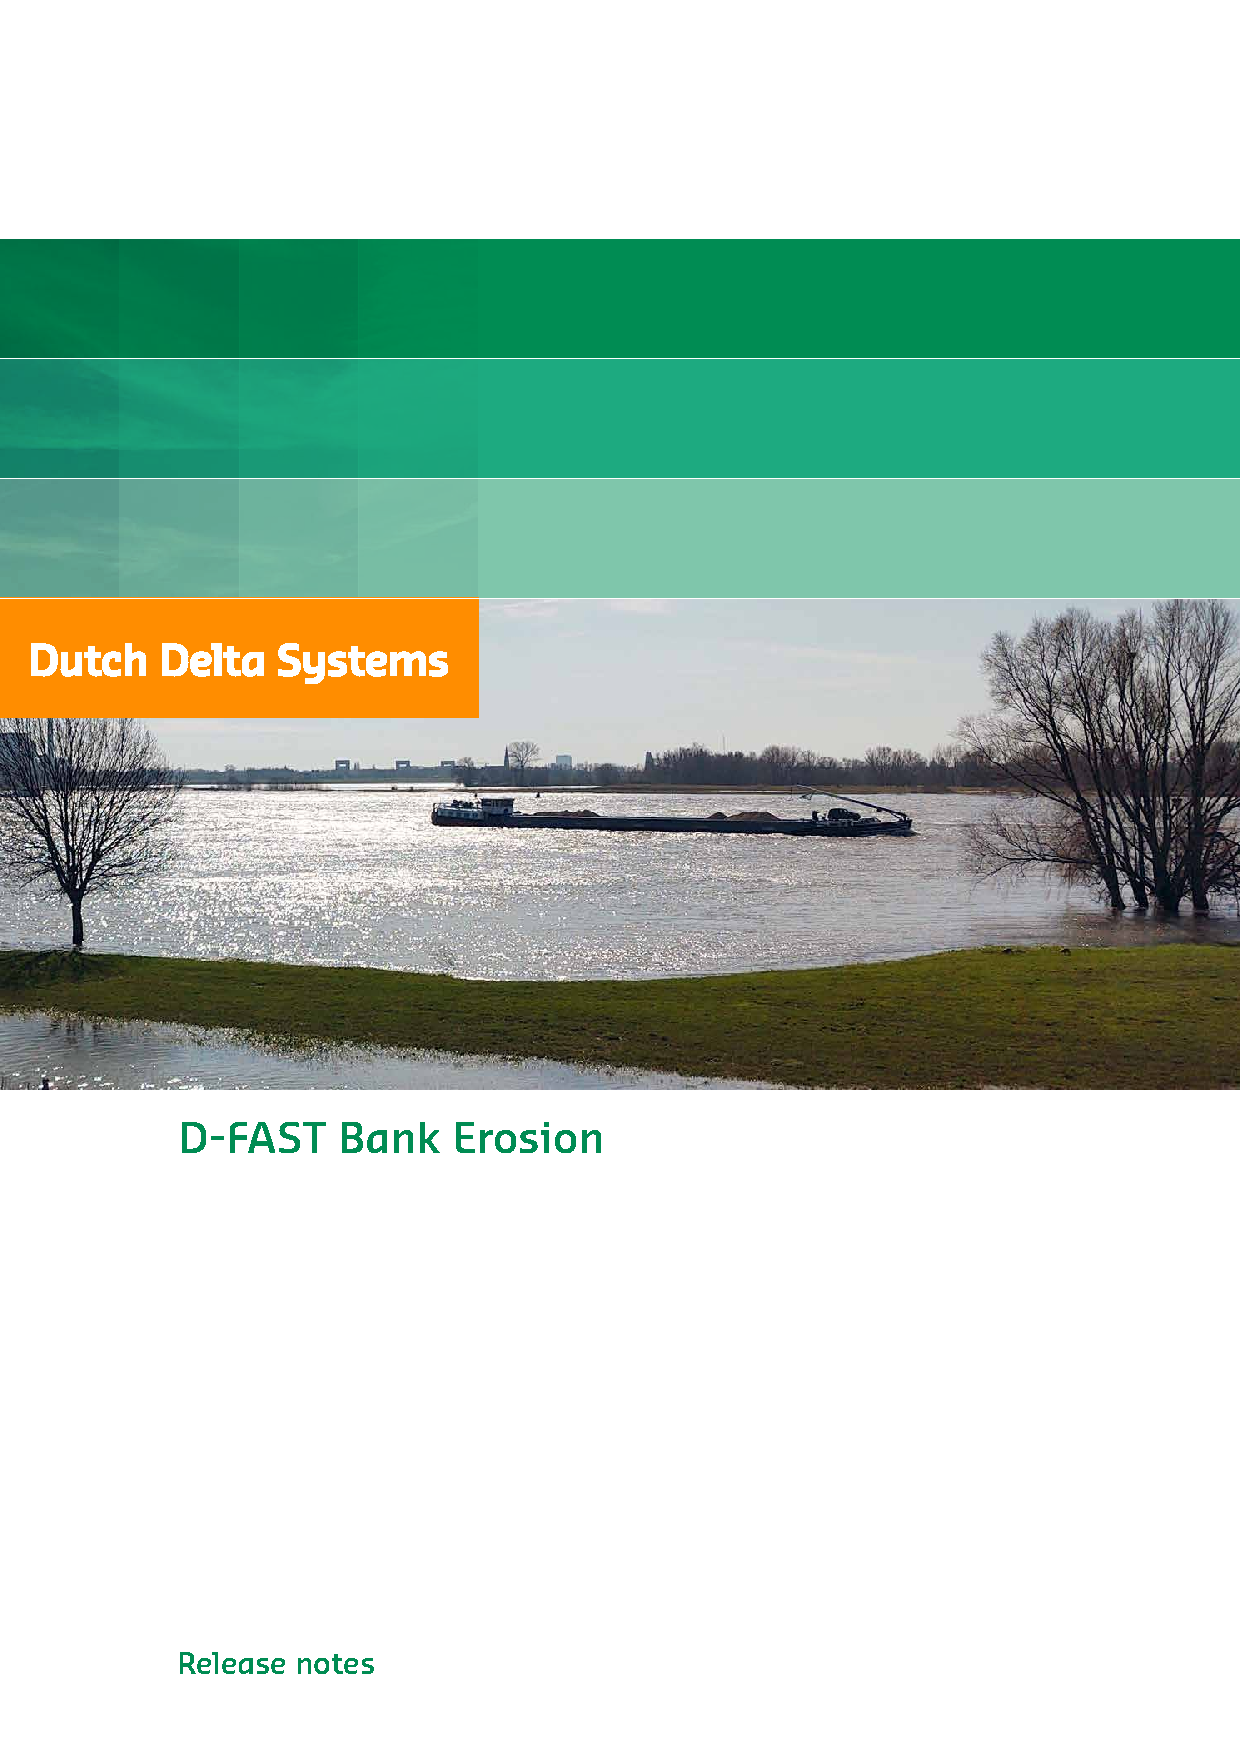
\includepdf[pages=1, offset=72 -70]{cover/D-FAST-omslag-D-FAST Bank Erosion-RN.pdf} % links-rechts past precies
\cleardoublepage
\title{D-FAST\\ Bank Erosion \dfbeversion}
\subtitle{}
\manualtype{Release Notes}
%\distribution{Released for: \newline \phantom{M} \dfbe version 3.0 or higher}
\version{\the\year.\the\month}

\author{ }

\setgitdirectory{../.git}
\deltarestitle

%------------------------------------------------------------------------------
\chapter{Introduction}
\section{Release contents}

\begin{tabular}{ll}
Description: & \dfastbe \\
Version: & \dfbeversion \\
Status & release
\end{tabular}

\fbox{%
\parbox{\textwidth}{%
\dfastbe version 3 is the successor of \dfastbe version 2 and WAQBANK.
The tool requires the result of a \dflowfm computation for a given set of flow conditions.
}}

\section{Compatibility}
\dfastbe is compatible with \dhydrosuite 2025.02.

\section{Installation}
\dfastbe is distributed as a plain zip-file.
The installation procedure is described in the \dfastbe, User Manual.

\section {Documentation list}
The following documentation is distributed with this release:

\begin{itemize}
	\item \dfastbe, Release notes (this document)
	\item \dfastbe, User Manual
	\item \dfastbe, Technical Reference Manual
%	\item \dfastbe, Validation Document
\end{itemize}

\chapter{Release summary}

\section{Version 3.0.0}

\subsection{Key changes summary}
This is a completely revised release, where the maintainability has been enhanced by improving the readability of the code, extend the testbench resulting in a (so-called) code-coverage of above 80\% and monitor code quality statistics during software maintenance.

The results are the same as those of the previous release \dfbe 2.3.1.

%Apart from the above, the following changes are worth mentioning:
%\begin{itemize}
%	\item Complete overview of analysis settings included in the report.
%	\item The tool is no longer supported in the Dutch language.
%	\item The WAQMORF compatible \keyw{cli} mode is no longer supported.
%	\item Configuration files of \dfmi version 2 are no longer supported by the GUI.
%\end{itemize}

\subsection{Known issues}

The known issues are:

\begin{itemize}
	\item none
\end{itemize}

\subsection{Overview of the resolved issues}

As this release is focused on maintainability, most changes are not relevant for the end user. Here follows a list of resolved issues since the release of version 2.3.1, which are relevant for the end user:

\begin{adjustbox}{left=-0.25cm}
	\begin{tabular}{ l l } 
		issue & description / summary\\ \hline
		DFAST-304 & Security issue: dependency on tornado \\
		DFAST-215 & Add cover pages to the documentation (UM, TRM and RelNotes) \\
	\end{tabular}
\end{adjustbox}

%------------------------------------------------------------------------------
\pagestyle{empty}
\cleardoublepage
\mbox{}
\includepdf[pages=2, offset=-72 -70]{cover/D-FAST-omslag-D-FAST Bank Erosion-RN.pdf} % links-rechts past precies
\end{document}
